\graphicspath{{chapters/08/}}
\chapter{Quantum computing}

\section{Qubits}
We can consider a quantum Hamiltonian $\hat{H_0}$ that describes a two-level system.
We can represent it with the same mathematical representation of spin even if it's not spin.
\begin{multicols}{2}
	\begin{itemize}
		\item $\ket{0}=\begin{pmatrix}1\\0\end{pmatrix}$
		\item $\ket{1}=\begin{pmatrix}0\\1\end{pmatrix}$
	\end{itemize}
\end{multicols}

With: $\hat{H_0}=-h\hat{\tau_x}$ and $\hat{\tau}_x$ Pauli matrix operator:

$$\hat{\tau_x}=\begin{pmatrix}0&1\\1&0\end{pmatrix}$$

Then:

$$\hat{H_0}=-h\begin{pmatrix}0&1\\1&0\end{pmatrix}$$

	\subsection{State of the Hamiltonian}
	The objective is to find:

	\begin{multicols}{2}
		\begin{itemize}
			\item$\ket{\hat{\Omega}}=\ket{\text{Ground state of }\hat{H_0}}$
			\item$\ket{\hat{\Sigma}}=\ket{\text{First excited state of }\hat{H_0}}$
		\end{itemize}
	\end{multicols}

	To find the possible states of the Hamiltonian first $\hat{H_0}\ket{\phi}=E\ket{\phi}$ is solved:

	\begin{align*}
		\det(H-\lambda \mathbb{1})&=0\\
		\det\begin{pmatrix}-\lambda&-h\\-h&-\lambda\end{pmatrix}&=0\\
		\lambda^2-h^2&=0 \rightarrow \lambda=\pm h
	\end{align*}

	$-h$ and $+h$ are the two possible energy eigenvalues and correspond to the ground state and first excited state, respectively.

		\subsubsection{Ground state}
		The ground state is computed: $E_\Omega=-h$

		$$\ket{\Omega}=\begin{pmatrix}a\\b\end{pmatrix}\rightarrow-h\begin{pmatrix}0&1\\1&0\end{pmatrix}\begin{pmatrix}a\\b\end{pmatrix}=-h\begin{pmatrix}a\\b\end{pmatrix}$$

		This is a two-variables system and can be resolved as such:

		$$\begin{cases}-ha=-ha\\-hb=-hb\end{cases}\rightarrow a=0\, \text{and}\, b=1\, \text{or}\, a=1\, \text{and}\, b=0$$

		$\ket{\Omega}$ can be rewrited as:

		$$\ket{\Omega}=\frac{1}{\sqrt{2}}\ket{1}+\frac{1}{\sqrt{2}}\ket{0}$$

		And since $\ket{1}=\begin{pmatrix}0\\1\end{pmatrix}$, the ket have to be normalized to get the $\begin{pmatrix}1\\1\end{pmatrix}$ that is the final result.
		$\ket{\Omega}$ is a quantum superposition of states.

		\subsubsection{First excited state}
		The first excited state: $E_\Sigma=+h$:

		$$[\ket{\Sigma}=\begin{pmatrix}a\\b\end{pmatrix}\rightarrow-h\begin{pmatrix}0&1\\1&0\end{pmatrix}\begin{pmatrix}a\\b\end{pmatrix}=+h\begin{pmatrix}a\\b\end{pmatrix}$$

		From this linear system we obtain the formulation for the first excited state.

		$$\ket{\Sigma}=\frac{1}{\sqrt{2}}\ket{1}-\frac{1}{\sqrt{2}}\ket{0}$$

		\subsubsection{Conclusion}
		Each of these two quantum states, $\ket{\Omega}$ and $\ket{\Sigma}$, represent a \textbf{qubit} that is in a linear superposition of states.\\

\subsection{Adiabatic Quantum Computing}
Putting energy in the system changes the probability of the particle of being still in a ground state.
The particle may be found in an excited state.
This doesn't happen if the system is switched in a slow manner and becomes an adiabatic system.
Doing so, according to the adiabatic system the system never ends up in an excited state and the transition is more likely to occur at time when $\Delta E$ is at its lowest.

	\subsubsection{Ground state of an arbitrary complex Hamiltonian}
	If $\hat{H_f}$ is complicated enough such that its ground state cannot be known, starting from $\hat{H_0}$ ground state and letting the system evolve in an adiabatic way to reach $\hat{H_f}$, $\hat{H_f}$ will reach the ground state spontaneously.
	Measuring the final state many times allows to discover the ground state of $\hat{H_f}$.

	\subsubsection{Final wave function through qubits}
	The final wavefunction can be obtained by means of qubits.
	Qubits are two level-systems that can thus have two levels of energy for which the two ground states are known.

\begin{figure}[htbp!]
	\centering
	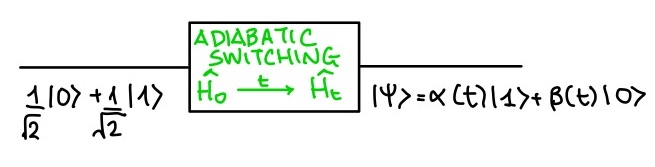
\includegraphics[scale=0.30]{img_10}
\end{figure}

The final solution can be computed by knowing the amount of values of $\alpha(t)$ and $\beta(t)$.
The time needed for the computation depends on:

\begin{multicols}{2}
	\begin{itemize}
		\item Triviality of the problem.
		\item The number of qubits $(n)$.
		\item The number of states ($2^n$).
		\item $\Delta E$.
	\end{itemize}
\end{multicols}

The time of computation depends on the function that regulated $\Delta E$ and corresponds to the clock of classical computers.

\section{Two qubits system}
Two qubits systems are interacting quantum systems.

	\subsection{Hamiltonian}
	The objective is to solve the Hamiltonian in the form:

	$$\hat{H}=\mathbf{J}_{12}\hat{\tau_1^z}\hat{\tau_2^z}+h(\hat{\tau_1^z}+\hat{\tau_2^z})$$

	This is a two-particles Hamiltonian that depends on the interaction of the two spins.
	If one of the two is down, $\hat{H}$ becomes negative and the energy is lowered.
	Hence I have a more favourable system.
	This can be obtained with a magnet that can properly align spins in order to have an overall negative energy.
	Implicitly, the Hamiltonian should be:

	$$\hat{H}=\mathbf{J}_{12}\hat{\tau_1^z}\hat{\tau_2^z}+h(\hat{\tau_1^z}\hat{\mathbb{1}_z}+\hat{\mathbb{1}_z}\hat{\tau_2^z})$$

	When using an operator on a particle, the other is multiplied by the identity matrix.

	$$\hat{\tau_1^z}\otimes\hat{\tau_2^z}=\begin{pmatrix}1&0&0&0\\0&-1&0&0\\0&0&-1&0\\0&0&0&1\end{pmatrix}\\hat{\tau_1^z}\otimes\hat{\mathbb{1}_z}=\begin{pmatrix}1&0&0&0\\0&1&0&0\\0&0&-1&0\\0&0&0&-1\end{pmatrix}\hat{\mathbb{1}^z}\otimes\hat{\tau_2^z}=\begin{pmatrix}1&0&0&0\\0&-1&0&0\\0&0&1&0\\0&0&0&-1\end{pmatrix}$$

	The Hamiltonian then becomes:

	$$\hat{H}=\mathbf{J}_{12}\begin{pmatrix}1&0&0&0\\0&-1&0&0\\0&0&-1&0\\0&0&0&1\end{pmatrix}+h\begin{pmatrix}2&0&0&0\\0&0&0&0\\0&0&0&0\\0&0&0&-2\end{pmatrix}=\begin{pmatrix}\mathbf{J}_{12}+2h&0&0&0\\0&-\mathbf{J}_{12}&0&0\\0&0&-\mathbf{J}_{12}&0\\0&0&0&-2h+\mathbf{J}_{12}\end{pmatrix}$$

	Each of the eigenvalues of the matrix can represent an eigenvector.

	\subsection{Quadratic unconstrained binary optimization problem}
	Suppose we have a function defined as a quadratic function of binary variables:

	$$T=\sum_{i,j=1}^N O_{ij}x_ix_j+\sum_i^N U_ix_i \text{ with } x_i\in \{0,1\} \text{ and } O_{ij},U_i\in \mathbb{R}$$

	The problem is finding the configuration of binary variables that minimises $T$.
	This is a discrete optimization problem that is called \textbf{Quadratic Unconstrained Binary Optimization (QUBO)} problem.
	We can reduce the two-particle problem to a QUBO problem.
	By definition $\hat{\tau_i^z}=2x_i-1$.
	When \[\begin{matrix}x_i=0&\hat{\tau_i^z}=-1\\x_i=1&\hat{\tau_i^z}=+1 \end{matrix}\]
	We can write the function $T$ as

	$$T=\sum_{i,j=1}^N \mathbf{J_{ij}}\tau_i^z\tau_j^z+\sum_i^N h_i\tau_i^z$$

	That is similar to the original Hamiltonian.
	This is the total number of combination of $2^N$.
	Values of $T$ are encoded in the Hamiltonian.
	Results of finding the minimum of $T$ and $\hat{H}$ are the same because the minimum value of the ground state corresponds to the ground eigenstate.
	The qubits corresponding to the ground eigenstate (eigenvectors) can be obtained from classical $T$ but not as a superposition.

	\subsection{Entangled states}
	Entangled states can be created by imposing a different spin direction on the particles.

	$$\hat{H}=\mathbf{J}_{12}\hat{\tau_1^z}\hat{\tau_2^z}+h(\hat{\tau_1^x}\hat{\mathbb{1}_x}+\hat{\mathbb{1}_x}\hat{\tau_2^x})$$
	$$\hat{\tau_1^x}\otimes\hat{\mathbb{1}_x}=\begin{pmatrix}0&0&1&0\\0&0&0&1\\1&0&0&0\\0&1&0&0\end{pmatrix}\hat{\mathbb{1}^x}\otimes\hat{\tau_2^x}=\begin{pmatrix}0&1&0&0\\1&0&0&0\\0&0&0&1\\0&0&1&0\end{pmatrix}\hat{H}=\begin{pmatrix}\mathbf{J}_{12}&h&h&0\\h&-\mathbf{J}_{12}&0&h\\h&0&-\mathbf{J}_{12}&h\\0&h&h&\mathbf{J}_{12}\end{pmatrix}$$

	The ground state is a vector correspondent to

	$$\begin{pmatrix}1\\0\\-\frac{\sqrt{4h^2+\mathbf{J}^2}+\mathbf{J}}{2h}\\1 \end{pmatrix}=\ket{0\,0}-\frac{\sqrt{4h^2+\mathbf{J}^2}+\mathbf{J}}{2h}\ket{1\,0}+\ket{1\,1}$$

	Where $c=\frac{\sqrt{4h^2+\mathbf{J}^2}+\mathbf{J}}{2h}$.
	Let the normalization factor:

	$$\frac{(1^2+c^2+1^2)}{N}=1 \rightarrow N=2+c^2$$

	$$G.S.=\frac{1}{\sqrt{2+c^2}}(\ket{0\,0}-c\,\ket{1\,0}+\ket{1\,1})$$

	Fix $c=1$ so the ground state becomes:

	$$G.S.= \frac{1}{\sqrt{3}}(\ket{0\,0}-\ket{1\,0}+\ket{1\,1})$$

	Compute the probability for $q_2=1$.
	$q_2$ can appear in two different states:

	\begin{align*}
		P_{1 1}&=\frac{1}{3}(\braket{1\,1\,|\,0\,0}-\braket{1\,1\,|\,1\,0}+\braket{1\,1\,|\,1\,1})^2=\bigg(\frac{1}{\sqrt{3}}\bigg)^2=\frac{1}{3}\\
		P_{0 1}&=\frac{1}{3}(\braket{0\,1\,|\,0\,0}-\braket{0\,1\,|\,1\,0}+\braket{0\,1\,|\,1\,1})^2=0
	\end{align*}

	This latter state never appears.
	The state is overall entangled because if $q_1=0$ the wave function collapses into $q_2=0$.
	If $q_1=1$, $q_2$ doesn't collapse because it can be either $q_2=0$ or $q_2=1$ with $50\%$ probability.
	$q_2$ is in a linear superposition of states if $q_1=1$.

\section{Quantum circuits}
Quantum circuits are models for \textbf{quantum computation},
where a computation is a sequence of quantum gates, measurements, and initialization of qubits to known values.
Circuits are written such as the horizontal axis is time and they are read from left to right.
Horizontal lines represent qubits, doubled lines are classical bits.
The items that connect the elements represents the operations performed on qubits.

	\subsection{Elementary logic gates}
	The elementary logic gates are model of computation or physical electronic devise that implements a boolean function on one or more binary input.
	They are irreversible: the input cannot be recovered from the output.

	\subsection{Universaility}
	Quantum computers can achieve universality, the complete conversion of an input of an arbitrary set of items into a corresponding output.
	Usually in quantum computation the output is a rotation of the input, all the operations used to perform such rotation $f(x)$ on input $x$ can be expressed as a single unitary matrix, for example

	$$U=\sum_j\ket{f(x)}\bra{x}$$

	The ability to implement any unitary matrix would mean the achievement of universality in the sense of standard digital computers.
	A strictly physical example would be the simulation of the dynamics of a system, where the time evolution is the unitary matrix and the Hamiltonian is the associated hermitian matrix.
	Achieving any unitary matrix would therefore correspond to simulating any time evolution, and engineering the effects of any Hamiltonian.

	\subsection{Quantum logic gates}
	Quantum logic gates are reversible unitary transformations on at least one qubit.

		\subsubsection{Qubits}
A qubit (the quantized version of classical \textit{n}-bit space $\{0,1\}^n$) is the Hilbert space $H_{QB(n)}=L^2(\{0,1\}^2)$, that can be interpreted as a linear combination or superposition of classical bit strings.
$H_{QB(n)}$ is a vector space over the complex numbers of dimension $2^n$ and elements of this vector space are possible state of \textit{n}-qubits quantum registers.
Quantum logic gates require a reversible function called unitary mapping which is linear transformation of a complex inner product space that preserves the Hermitian inner product.

	\subsection{Types of quantum circuits}
	There are three main types of quantum circuits:

	\begin{multicols}{2}
		\begin{itemize}
		\item \textbf{Phase gate (S gate)}: single-qubit operation defined by the matrix $S=\begin{pmatrix}1&0\\0&i \end{pmatrix}$, it represents a $90^\circ$ rotation around the $z$-axis.
		\item \textbf{Hadamard gate}: single-qubit operation that maps the basis state $\ket{0}$ to $\frac{\ket{0}+\ket{1}}{\sqrt{2}}$ and $\ket{1}$ to $\frac{\ket{0}-\ket{1}}{\sqrt{2}}$ thus creates a superposition of the two basis states.
			It can be represented by the matrix $H=\frac{1}{\sqrt{2}}\begin{pmatrix} 1&1\\1&-1\end{pmatrix}$.
			It represents a $90^{\circ}$ rotation around the $y$-axis followed by a $180^{\circ}$ rotation around the $x$-axis.
		\item \textbf{CNOT gate}: two-qubit operation.
			The first qubit is the control qubit, the second qubit is the target qubit.
			This gate leaves the control qubit unchanged and performs a Pauli-X gate on the target qubit if control is $\ket{1}$.
			If control is $\ket{0}$ the target qubit is unchanged.
			The CNOT gate is represented by the matrix $C_{NOT} = \begin{pmatrix}1&0&0&0\\0&1&0&0\\0&0&0&1\\0&0&1&0 \end{pmatrix}$
		\end{itemize}
	\end{multicols}

	\begin{figure}[htbp!]
		\centering
		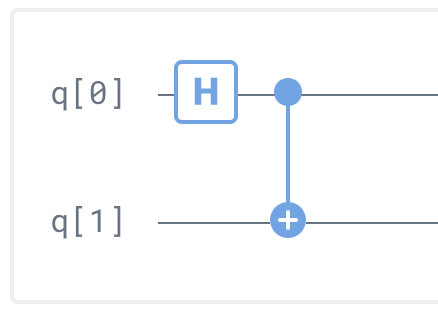
\includegraphics[scale=0.30]{img_11}
	\end{figure}

	The figure represents the execution of Hadamard gate on qubit 0 to create a superposition state and then the execution of CNOT gate to create an entangled state of the two qubits.

	\subsection{Prove that Hadamard gate is the reverse of itself}

	\begin{align*}
		H&=\frac{1}{\sqrt{2}}\begin{pmatrix}1&1\\1&-1\end{pmatrix}\,\,\ket{0}=\begin{pmatrix}1\\0\end{pmatrix}\,\,\ket{1}=\begin{pmatrix}0\\1\end{pmatrix}\\
		H\,\ket{0}&=\frac{1}{\sqrt{2}}\begin{pmatrix}1&1\\1&-1\end{pmatrix}\begin{pmatrix}1\\0\end{pmatrix}=\frac{1}{\sqrt{2}}\begin{pmatrix}1+0\\1+0\end{pmatrix}=\begin{pmatrix}1/\sqrt{2}\\1/\sqrt{2}\end{pmatrix}\\
		H\,(H\,\ket{0})&=\frac{1}{\sqrt{2}}\begin{pmatrix}1&1\\1&-1\end{pmatrix}\begin{pmatrix}1/\sqrt{2}\\1/\sqrt{2}\end{pmatrix}=\frac{1}{\sqrt{2}}\begin{pmatrix}1/\sqrt{2}+1/\sqrt{2}\\1/\sqrt{2}-1/\sqrt{2}\end{pmatrix}=\frac{1}{\sqrt{2}}\begin{pmatrix}2/\sqrt{2}\\0\end{pmatrix}=\begin{pmatrix}1\\0\end{pmatrix}
	\end{align*}

	It's pointless to put two Hadamard gates in a row from a mathematical point of view.
	From a physical point of view it means that I am restoring the cat in an aline/dear definite state that is technically not possible.

	\subsection{Example of a $HC_{NOT}$}
	Application of the two gates on different entangled states of qubits $\ket{0}$ and $\ket{1}$.

	\begin{align*}
		C_{NOT}(H\,\ket{0\,0})&=C_{NOT}(H\,\ket{0}\otimes\ket{0})=C_{NOT}\bigg(\frac{1}{\sqrt{2}}\begin{pmatrix}1&1\\1&-1\end{pmatrix}\begin{pmatrix}1\\0\end{pmatrix}\otimes\begin{pmatrix}1\\0\end{pmatrix}\bigg)=\\
													&=C_{NOT}\bigg(\frac{1}{\sqrt{2}}\begin{pmatrix}1\\1\end{pmatrix}\otimes\begin{pmatrix}1\\0\end{pmatrix}\bigg)=\\
													&=C_{NOT}\frac{1}{\sqrt{2}}\begin{pmatrix}1\\0\\\mathcolorbox{yellow}{1}\\\mathcolorbox{yellow}{0}\end{pmatrix}=\frac{1}{\sqrt{2}}\begin{pmatrix}1&0&0&0\\0&1&0&0\\0&0&0&1\\0&0&1&0\end{pmatrix}\begin{pmatrix}1\\0\\1\\0\end{pmatrix}=\\
													&=\frac{1}{\sqrt{2}}\begin{pmatrix}1+0+0+0\\0+0+0+0\\0+0+0+0\\0+0+1+0\end{pmatrix}=\frac{1}{\sqrt{2}}\begin{pmatrix}1\\0\\\mathcolorbox{yellow}{0}\\\mathcolorbox{yellow}{1}\end{pmatrix}=\\
													&=\frac{\ket{0\,0}+\ket{1\,1}}{\sqrt{2}}=\ket{\phi^+}
	\end{align*}
	As foreseen in the theory, the second qubit changes when the $C_{NOT}$ gate is applied.
	The result is an entangled state of the two qubits called Bell state.
	All Bell states resulting from the combinations are orthogonal to each other.

	$$\frac{\ket{0\,0}-\ket{1\,1}}{\sqrt{2}}=\ket{\phi^-}\,\,\frac{\ket{0\,1}+\ket{1\,0}}{\sqrt{2}}=\ket{\psi^+}\,\,\frac{\ket{0\,1}-\ket{1\,0}}{\sqrt{2}}=\ket{\psi^-}$$

	$$\braket{\psi^+\,|\,\psi^-}=0$$

\section{The Elitzur-Vaidman bomb tester}
The Elitzur-Vaidman bomb tester is a quantum mechanics thought experiment that uses interaction-free mechanism to verify that a bomb is functional without having to detonate it.
This experiment uses two characteristics of elementary particles: \textbf{nonlocality} and \textbf{wave-particle duality}.
The fundamentals of this experiment can be explained with an example: if we have two closed boxes and we know that in one of the two there is an object, by opening one and finding it empty, we know that the object is in the other one without opening it.
The particle, during the experiment, is in a superposition of states/locations, it can be anywhere in any moment.
The particle's wave can be collapsed by observing it to obtain its local information.
Information about previous positions of the particle can be obtained before the collapse and even in cases where the particle was never in those positions.

\begin{figure}[htbp!]
	\centering
	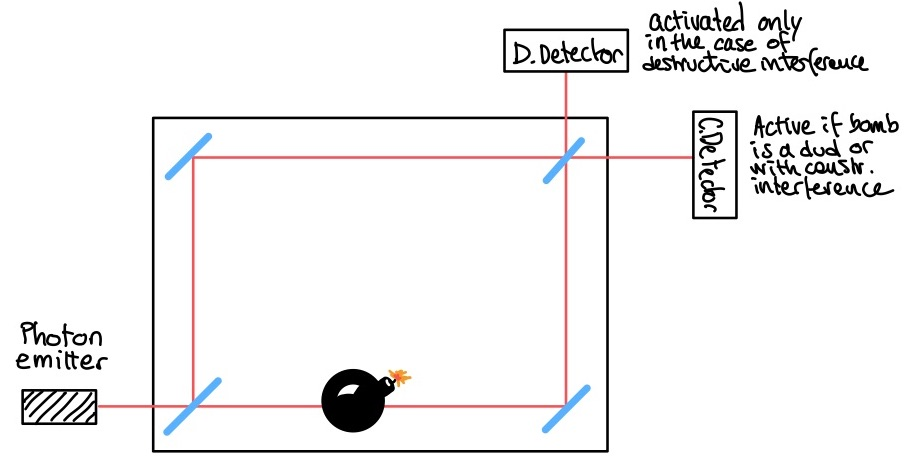
\includegraphics[scale=0.30]{img_12}
\end{figure}


	\subsection{Bomb not inserted}
When the photon is emitted and it reaches the first beam splitter, a superposition of states is created, the photon can either go to the upper path or to the lower path with a $50\%$ probability each.
The photon encounters two mirrors that reflect the beam and the two meet at a second beam splitter that directs the beam to two detectors with the same probability:

\begin{multicols}{2}
	\begin{itemize}
		\item C Detector: reached by the transmitted beam.
	Activated by the constructive interference of the two photons behaving as waves.
		\item D Detector: reached by the reflected beam.
	Never activated in normal conditions (destructive interference happens hence no signal)
	\end{itemize}
\end{multicols}

	\subsection{Dud bomb}
	When the bomb is dud, $C$ detector has a $100\%$ probability of detecting a signal.
	The superposition of states created by the first beam splitter create a constructive interference that is detected by $C$.
	In $D$ there is destructive interference so nothing is detected.

	\subsection{Bomb inserted and live}
	Three things may happen when the bomb is inserted and live:

	\begin{multicols}{2}
		\begin{itemize}
			\item $50\%$ the bomb explodes: The photon took the lower path and activated the bomb.
				The activation of the bomb can be considered as a collapse of the wave function, the photon never arrives at the detector and no signal is present.
			\item $25\%$ photon detected at $C$: The photon took the upper way and was transmitted by the second beam splitter.
			\item $25\%$ photon detected at $D$: The photon took the upper way and was reflected by the second beam splitter.
				The presence of a signal at detector $D$ is the only way to know whether the bomb is live without its explosion.
		\end{itemize}
	\end{multicols}
